\setcounter{chaptercntr}{3}

\sectionbreak {
	\gostTitleFont
	\redline
	\thechaptercntr . 
	ПРОЕКТИРОВАНИЕ АРХИТЕКТУРЫ СЕРВЕРНОЙ ЧАСТИ
	
}

\titlespace

\subsection*{ 
	\gostTitleFont
	\redline
	\thechaptercntr .\thesubchaptercntr \spc
	Разработка схемы взаимодействия микросервисов
} \addtocounter{subchaptercntr}{1}

\subtitlespace

{\gostFont
	
	\par \redline Проектирование серверной части приложения такси начинается с определения того, из каких компонентов она будет состоять и как эти компоненты будут между собой общаться. Исходя из результатов анализа, проведённого в предыдущих главах, было решено строить систему на основе микросервисной архитектуры. Логика тут простая: каждый крупный блок функциональности выносится в отдельный сервис, у каждого своя БД, и они общаются по сети. Это даёт гибкость в плане масштабирования и независимого развития отдельных частей системы [1].
	
	\par \redline В разрабатываемой системе можно выделить два типа сервисов: инфраструктурные и бизнесовые. К инфраструктурным относятся Eureka (для поиска и обнаружения сервисов), Config Server (хранилище общих настроек) и API Gateway (единая точка входа). Бизнесовых сервисов пять: сервис аутентификации, сервис пассажиров, сервис водителей, сервис поездок и сервис рейтинга. Каждый из них отвечает за свою область и имеет собственную БД. Схему того, как это всё связано, можно увидеть на рисунке 
	\thechaptercntr .\theimagecntr .
	
	\par \redline API Gateway работает на порту 8080. Он принимает все входящие запросы от клиентов, проверяет цифровые подписи и направляет запросы к нужным сервисам. Например, запросы на /api/v1/passengers/** идут в сервис пассажиров, на /api/v1/drivers/** - в сервис водителей, на /api/v1/rides/** - в сервис поездок. Все сервисы регистрируются в Eureka, поэтому gateway может обращаться к ним по именам, а система сама находит нужный сервис и распределяет нагрузку. Config-server, в свою очередь, хранит общие настройки для всех сервисов, и при старте каждый сервис получает конфигурацию оттуда.
	
	\par \redline Теперь про то, как сервисы общаются между собой. Тут используется два подхода: синхронный через HTTP-вызовы и асинхронный через систему обмена сообщениями. Синхронные вызовы применяются там, где нужно получить ответ прямо сейчас. Например, когда сервис аутентификации регистрирует нового пользователя, он сначала создаёт учётную запись, а потом через HTTP-запрос обращается к сервису пассажиров или сервису водителей, чтобы создать профиль. Другой пример: сервис поездок перед назначением водителя на заказ проверяет, что водитель существует и не занят. Все эти вызовы защищены: каждый сервис авторизуется как доверенное приложение, а не как конкретный пользователь.
	
	\par \redline Чтобы синхронные вызовы не ломали всю систему, если какой-то сервис временно недоступен, используются механизмы обработки ошибок: делается несколько повторных попыток, а при постоянных сбоях вызовы временно прекращаются, чтобы один упавший сервис не повалил всю систему [1].
	
	\begin{figure}[H]
		\centering
		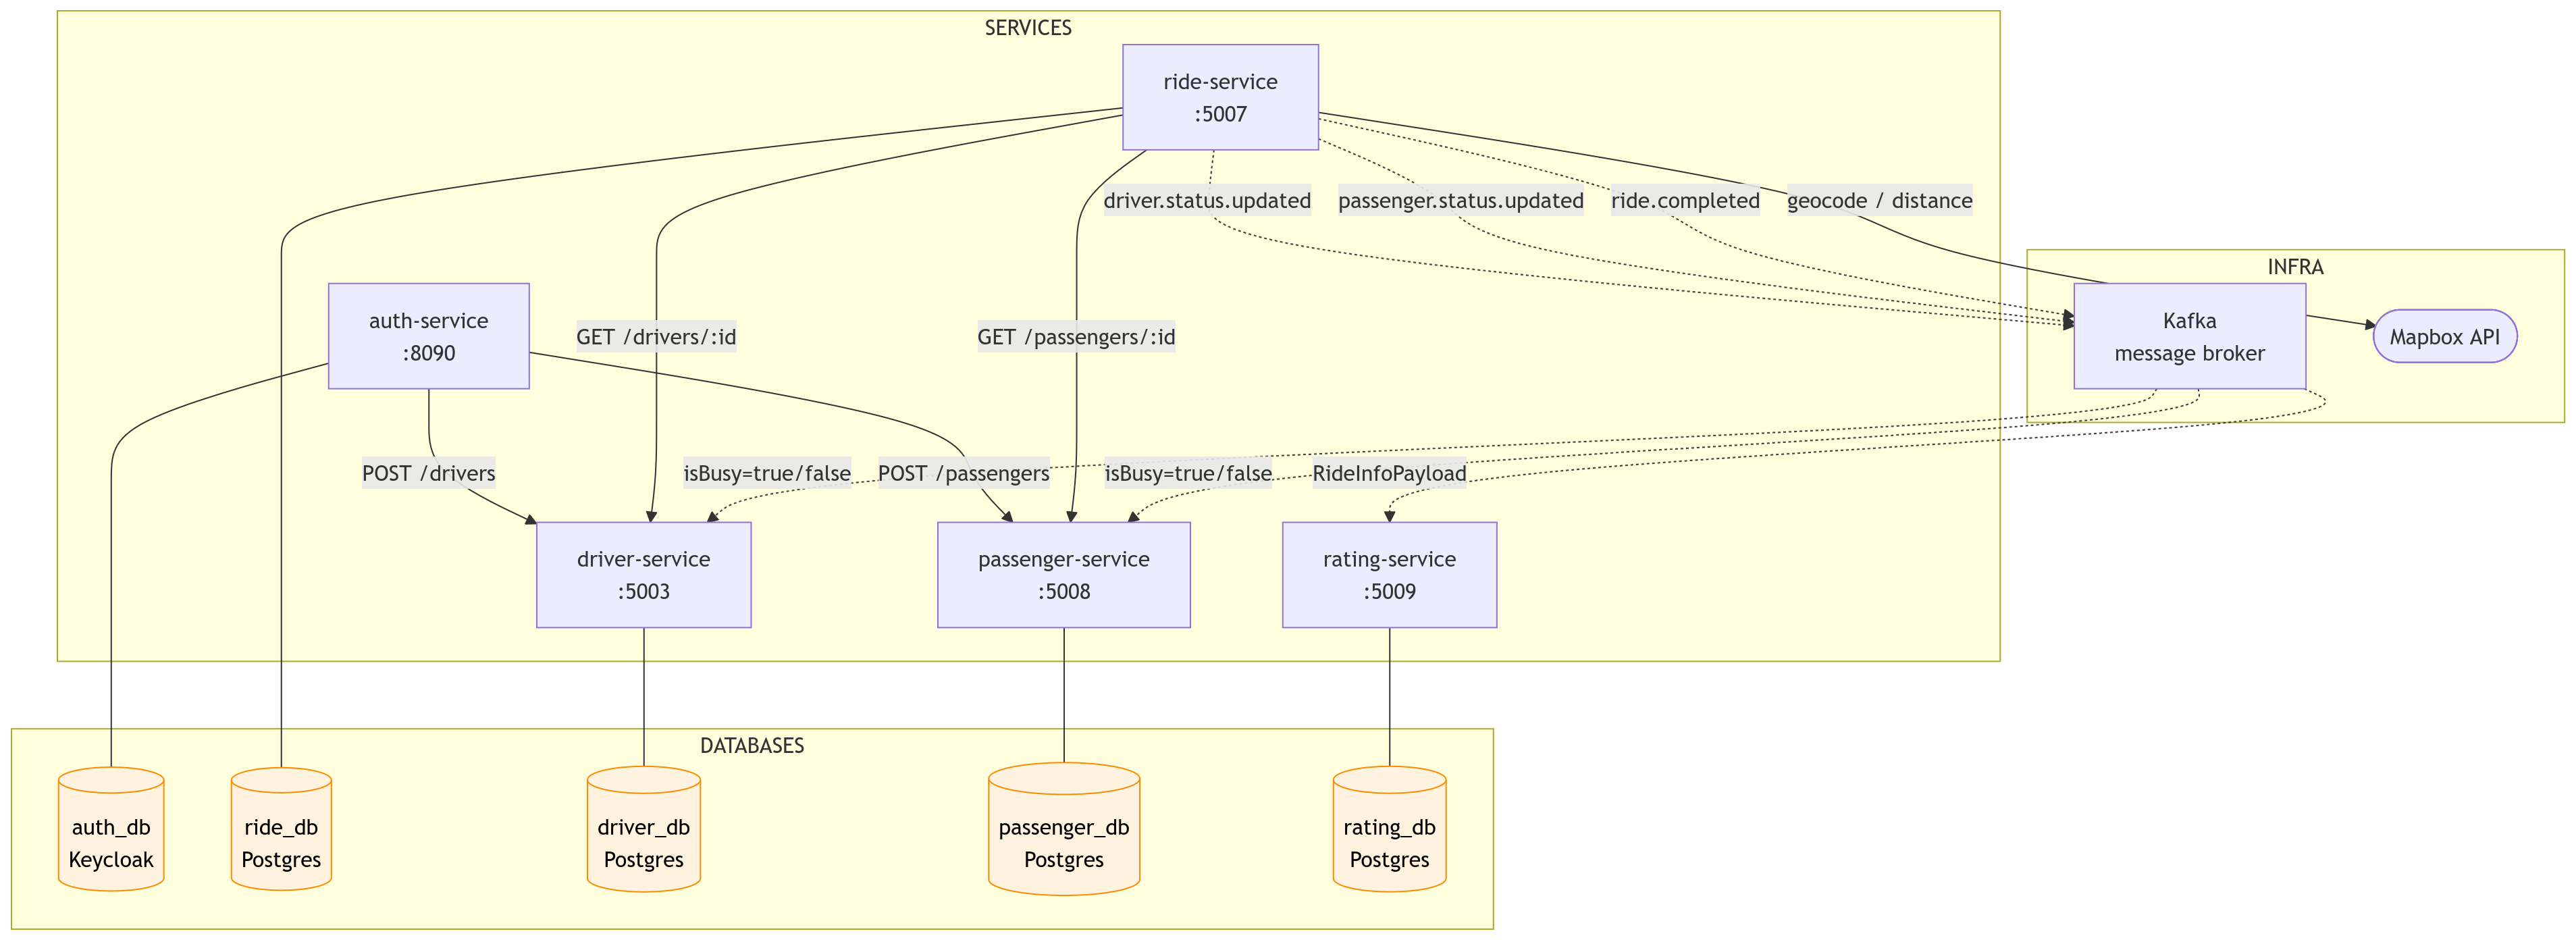
\includegraphics[width=700pt, angle=90]{images/microservice.png}
		\caption*{\gostFont Рисунок \thechaptercntr .\theimagecntr \spc {--} Схема взаимодействия микросервисов}
		\label{fig:microservices_diagramm}
	\end{figure} \addtocounter{imagecntr}{1}
	
	\par \redline Асинхронное взаимодействие используется для событий, где не нужно ждать ответа прямо сейчас. Например, при создании поездки меняется статус пассажира на "занят", при назначении водителя - статус водителя. Или когда поездка завершена - нужно сказать сервису рейтинга, что можно выставлять оценки. Для таких вещей сервис поездок отправляет сообщения через систему обмена сообщениями, а сервисы пассажиров, водителей и рейтинга получают эти сообщения и обрабатывают их.
	
	\par \redline Но тут есть нюанс: если отправить сообщение, а потом что-то пойдёт не так, данные могут разойтись. Чтобы такого не было, используется следующий подход: сначала данные сохраняются в БД вместе с изменением статуса поездки, а потом уже отправляются получателю. Если отправка не удалась - данные остаются в БД и будут отправлены при следующей попытке. Так гарантируется, что сообщение дойдёт хотя бы один раз [8].
	
	\par \redline Отдельно стоит сказать про авторизацию и аутентификацию. За это отвечает внешняя система управления доступом. Когда пользователь регистрируется или заходит через сервис аутентификации, тот связывается с этой системой, получает цифровой ключ доступа и передаёт его клиенту. Дальше клиент при каждом запросе прикладывает этот ключ. API Gateway проверяет ключ, достаёт оттуда идентификатор пользователя и передаёт его другим сервисам в специальном заголовке. Таким образом сервисы могут реализовать адрес /me, чтобы получить профиль текущего пользователя.
	
	\par
}

\titlespace

\subsection*{
	\gostTitleFont
	\redline
	\thechaptercntr .\thesubchaptercntr \spc
	Проектирование структуры базы данных
} \addtocounter{subchaptercntr}{1}

\titlespace

{\gostFont
	
	\par \redline У каждого бизнес-сервиса в системе своя БД. Такой подход снижает связанность: изменение схемы одного сервиса не затрагивает остальные [1]. Все изменения схемы отслеживаются с помощью Liquibase - инструмента миграций, который хранит список изменений (changelog) непосредственно в проекте. При запуске сервиса Liquibase проверяет, какие миграции уже применены, и выполняет только новые. Это гарантирует, что схема БД всегда соответствует версии кода, а при необходимости миграцию можно откатить.
	
	\par \redline Связи между основными сущностями системы показаны на ER-диаграмме (рисунок \thechaptercntr .\theimagecntr). В системе выделено четыре БД - по одной на бизнес-сервис. В сервисе водителей две таблицы: driver и car. В driver хранятся имя, фамилия, электронная почта, телефон, пол, флаги активности и занятости, а также привязка к учётной записи Keycloak. В car - цвет, марка, номер автомобиля, флаг активности и внешний ключ к таблице driver. Связь между таблицами типа "один ко многим": водитель может владеть несколькими автомобилями.
	
	\begin{figure}[H]
		\centering
		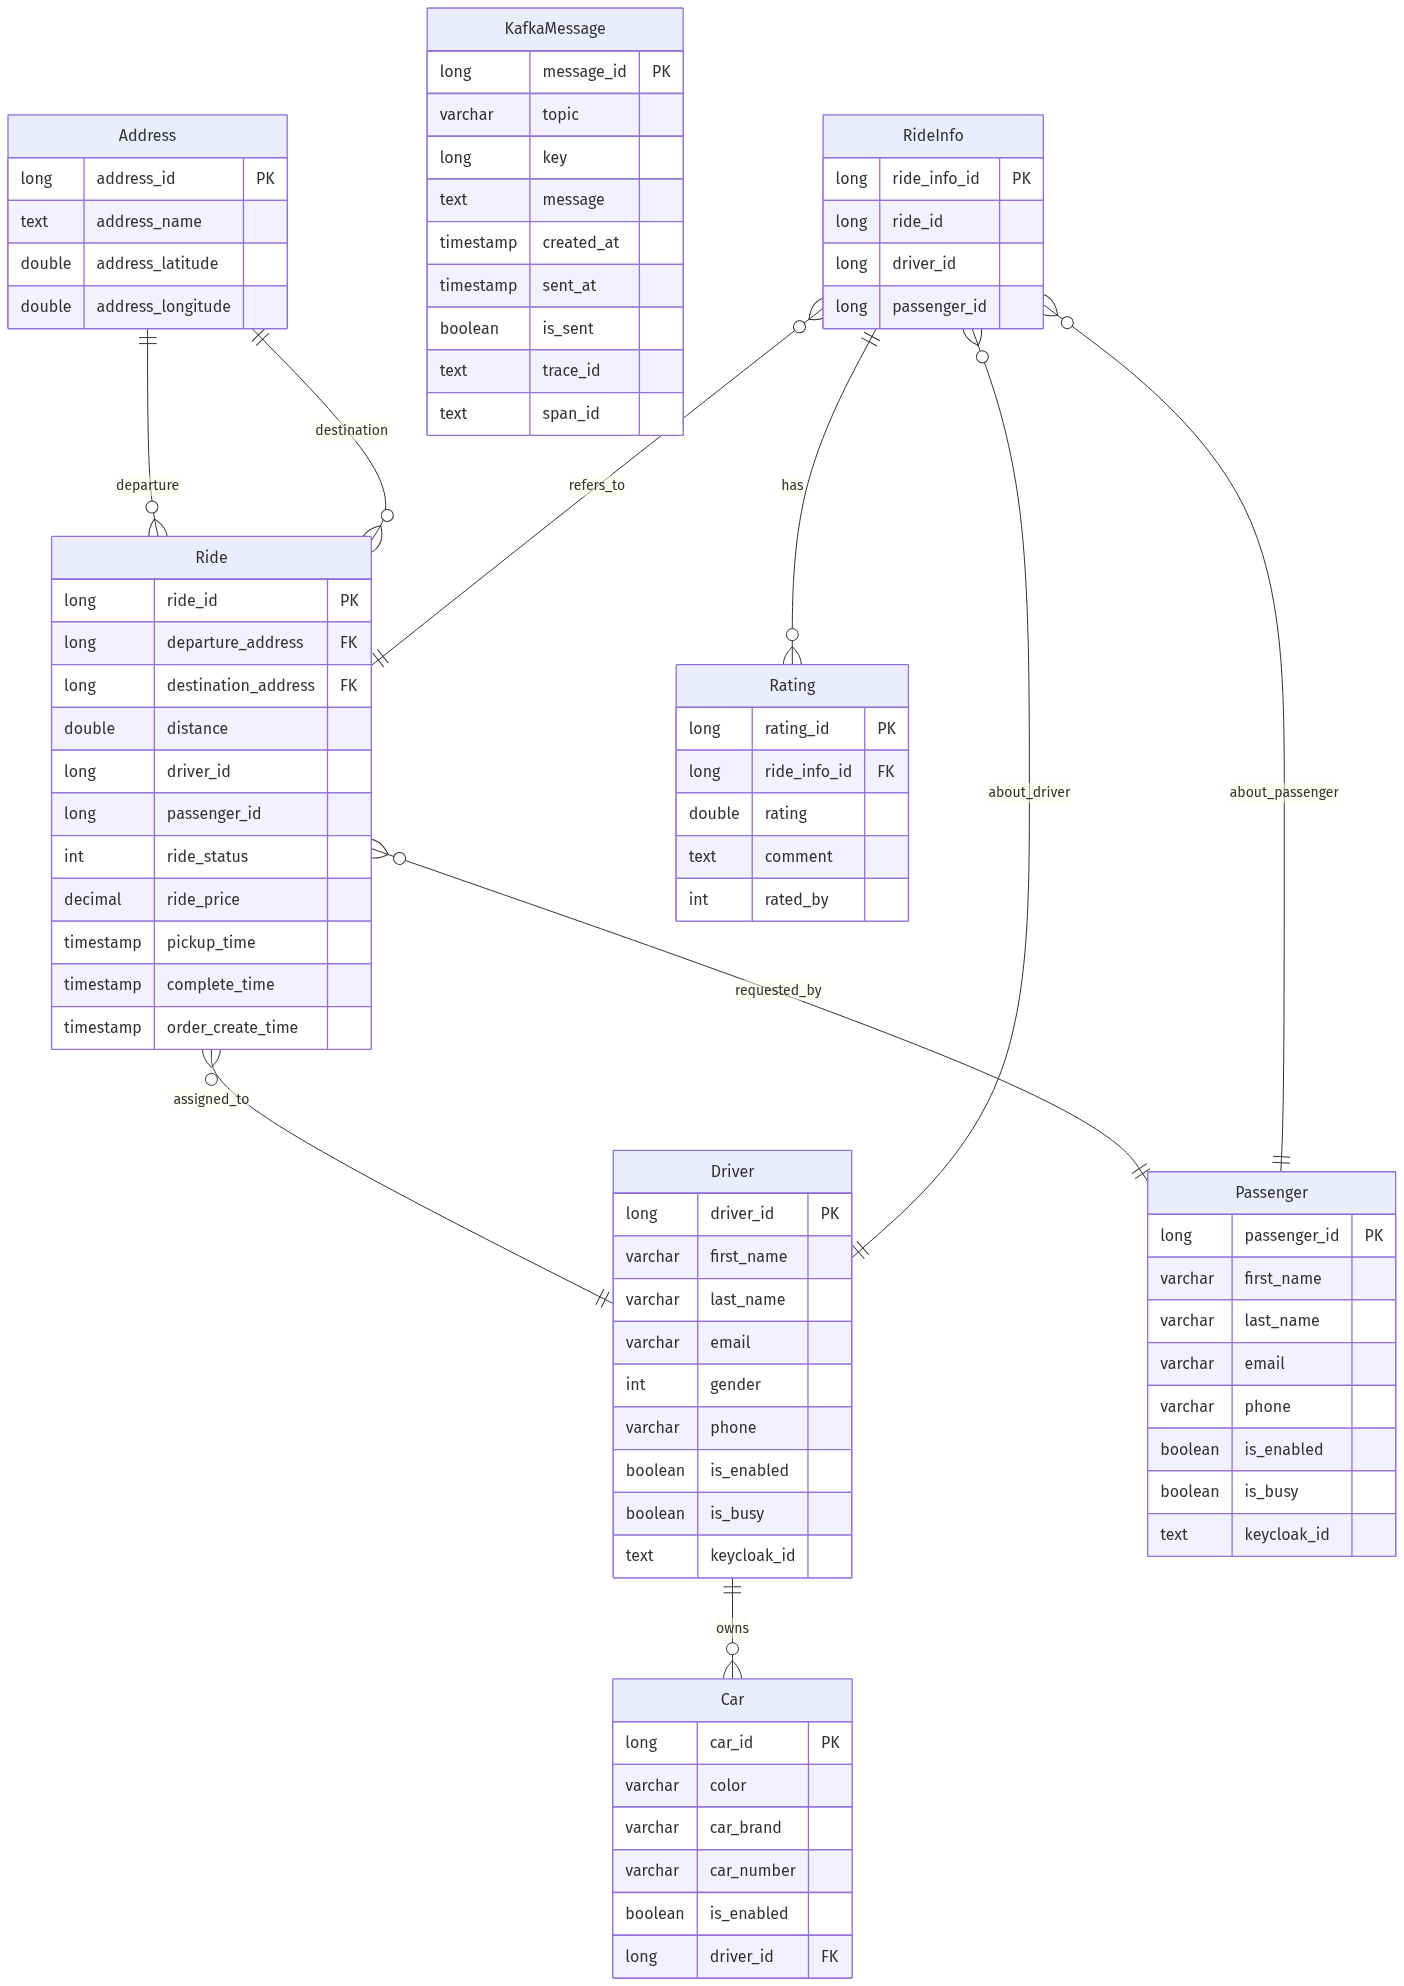
\includegraphics[width=490pt]{images/er_diagram.png}
		\caption*{\gostFont Рисунок \thechaptercntr .\theimagecntr \spc {--} ER-диаграмма базы данных}
		\label{fig:er_diagram}
	\end{figure} \addtocounter{imagecntr}{1}

	\par \redline Сервис пассажиров содержит единственную таблицу passenger с аналогичным набором полей: имя, фамилия, email, телефон, флаги активности и занятости, keycloak\_id.
	
	\par \redline Наиболее насыщенной является БД сервиса поездок, включающая таблицы ride, address и kafka\_messages. Центральная таблица ride содержит: внешние ключи к таблице address (адреса отправления и назначения), идентификаторы водителя и пассажира в виде логических ссылок (без ограничений на уровне СУБД, поскольку эти сущности хранятся в других БД), статус поездки (12 возможных состояний, хранятся числом и преобразуются в перечисление средствами ORM), цену, дистанцию в метрах и три временные метки - создания заказа, подачи автомобиля и завершения поездки.
	
	\par \redline Таблица address отвечает за хранение геоданных. В ней четыре поля: название адреса (строка), широта и долгота (тип double precision) и суррогатный ключ. Тип double precision обеспечивает точность, достаточную для задач городской навигации. Широта принимает значения от -90 до 90 градусов, долгота - от -180 до 180. Координаты проверяются на уровне приложения перед записью, что исключает сохранение некорректных данных. Для ускорения поиска по названию на поле address\_name создан индекс - это позволяет находить уже известные системе адреса без повторного обращения к картографическому сервису.
	
	\par \redline В текущей версии системы поиск ближайших водителей выполняется через внешний картографический сервис, а не через пространственные запросы к БД. Поэтому геоинформационные расширения PostgreSQL, такие как PostGIS, пока не задействованы. Однако модель данных допускает их подключение в будущем: достаточно добавить столбец геометрического типа и заполнить его на основе уже имеющихся координат без изменения существующей структуры таблиц.
	
	\par \redline При создании поездки пользователь указывает адреса отправления и назначения. Сервис поездок направляет их в картографический сервис, получает координаты и сохраняет в таблицу address. Затем по паре координат через тот же сервис вычисляется расстояние в метрах. Чтобы снизить число обращений к внешнему сервису, результаты всех трёх операций кэшируются в Redis: кэшируется сам адрес (название вместе с координатами), результат геокодирования (преобразование названия в координаты) и расстояние между конкретной парой адресов.
	
	\par \redline Таблица kafka\_messages служит хранилищем исходящих сообщений. При изменении статуса поездки, требующем оповещения других сервисов (например, о занятости водителя или завершении поездки), сообщение сначала записывается в эту таблицу в рамках той же транзакции. Это гарантирует согласованность: если транзакция зафиксирована, то и данные поездки, и сообщение сохранены одновременно. Таблица содержит поля: топик, ключ (обычно идентификатор сущности), тело сообщения в JSON, время создания, время отправки и флаг is\_sent. На полях is\_sent и created\_at построен составной индекс для быстрого поиска неотправленных сообщений. Раз в секунду фоновая задача выбирает строки с is\_sent = false и публикует их в брокер сообщений, после чего помечает как отправленные. Если брокер временно недоступен, сообщения накапливаются в таблице и будут отправлены при следующем успешном цикле [8].
	
	\par \redline Поскольку сервис поездок может работать в нескольких экземплярах, фоновая задача отправки должна выполняться только на одном из них во избежание дублирования. Для этого задействован механизм распределённых блокировок ShedLock: перед запуском задача пытается захватить блокировку через служебную таблицу в той же БД. Если блокировка уже занята другим экземпляром, задача пропускает цикл. Раз в сутки срабатывает задача очистки, удаляющая сообщения, отправленные более суток назад, чтобы таблица не разрасталась.
	
	\par \redline Сервис рейтинга содержит таблицы ride\_info и rating. При получении сообщения о завершённой поездке создаётся запись в ride\_info с идентификаторами поездки, водителя и пассажира. После этого каждый участник может выставить оценку: в таблицу rating помещается строка со ссылкой на ride\_info, числовой оценкой (от 0 до 5), текстовым комментарием и признаком того, кто поставил оценку - пассажир или водитель. Средний рейтинг вычисляется динамически: берутся последние N оценок (по умолчанию 20) и рассчитывается среднее арифметическое.
	
	\par
}

\titlespace

\subsection*{ 
	\gostTitleFont
	\redline
	\thechaptercntr .\thesubchaptercntr \spc
	Разработка API и протоколов обмена данными
} \addtocounter{subchaptercntr}{1}

\titlespace

{\gostFont
	
	\par \redline API серверной части спроектирован в REST-стиле. Все запросы приходят на единый шлюз на порту 8080, а оттуда уже направляются к конкретным сервисам. Формат данных - JSON. Общая схема API показана в таблице \thechaptercntr .\thetablecntr .
	
	\topTablespace
	{\begin{Center}
			\par Таблица \thechaptercntr .\thetablecntr \spc {--} Маршрутизация API Gateway
			
			\begin{tabular}{|c|c|c|c|}
				\hline
				Путь & Сервис & Авторизация & Описание \\ \hline
				/auth/** & аутентификация & нет & Регистрация и вход \\ \hline
				/passengers/** & пассажиры & да & Работа с пассажирами \\ \hline
				/drivers/** & водители & да & Работа с водителями \\ \hline
				/cars/** & водители & да & Работа с машинами \\ \hline
				/rides/** & поездки & да & Управление поездками \\ \hline
				/ratings/** & рейтинг & да & Оценки и рейтинг \\ \hline
		\end{tabular} \end{Center}}
	\botTablespace \addtocounter{tablecntr}{1}
	
	\par \redline Сервис аутентификации отвечает за вход и регистрацию. У него есть открытые адреса: POST /signup (создание пользователя и его профиля), POST /signin (получение ключа доступа), POST /refresh (обновление ключа) и POST /logout (отзыв старого ключа). После регистрации сервис аутентификации через HTTP-запрос обращается к сервису пассажиров или сервису водителей, чтобы создать профиль.
	
	\par \redline Сервисы пассажиров и водителей предоставляют операции создания, чтения, обновления и удаления для своих записей. Помимо обычных адресов для работы с конкретными записями у них есть адрес /me, который возвращает профиль текущего пользователя по его идентификатору, полученному из специального заголовка. Это удобно для клиента - не нужно хранить внутренние идентификаторы. Также есть список всех записей с возможностью постраничного просмотра.
	
	\par \redline Самый интересный сервис с точки зрения API - это сервис поездок. Для начала поездки клиент отправляет POST /rides с указанием адреса отправления, назначения и своего ID. Система проверяет, что пассажир не занят, преобразует адреса в координаты через картографический сервис, считает дистанцию и цену (10 условных единиц за километр), создаёт поездку и сразу переводит её в статус ожидания водителя, отправляя сообщение о том, что пассажир занят.
	
	\par \redline Дальше поездка живёт по конечному автомату, который включает 12 возможных состояний и переходы между ними. Вот как выглядит полный жизненный цикл поездки: CREATED - WAITING\_FOR\_DRIVER - DRIVER\_ASSIGNED - ACCEPTED - \\ON\_THE\_WAY\_TO\_PASSENGER - PASSENGER\_PICKED\_UP - ON\_THE\_WAY - \\COMPLETED - PAYMENT\_PENDING - PAID - RATE. Из многих состояний можно отменить поездку (CANCELLED). Визуально диаграмма состояний показана на рисунке \thechaptercntr .\theimagecntr .

	\begin{figure}[H]
		\centering
		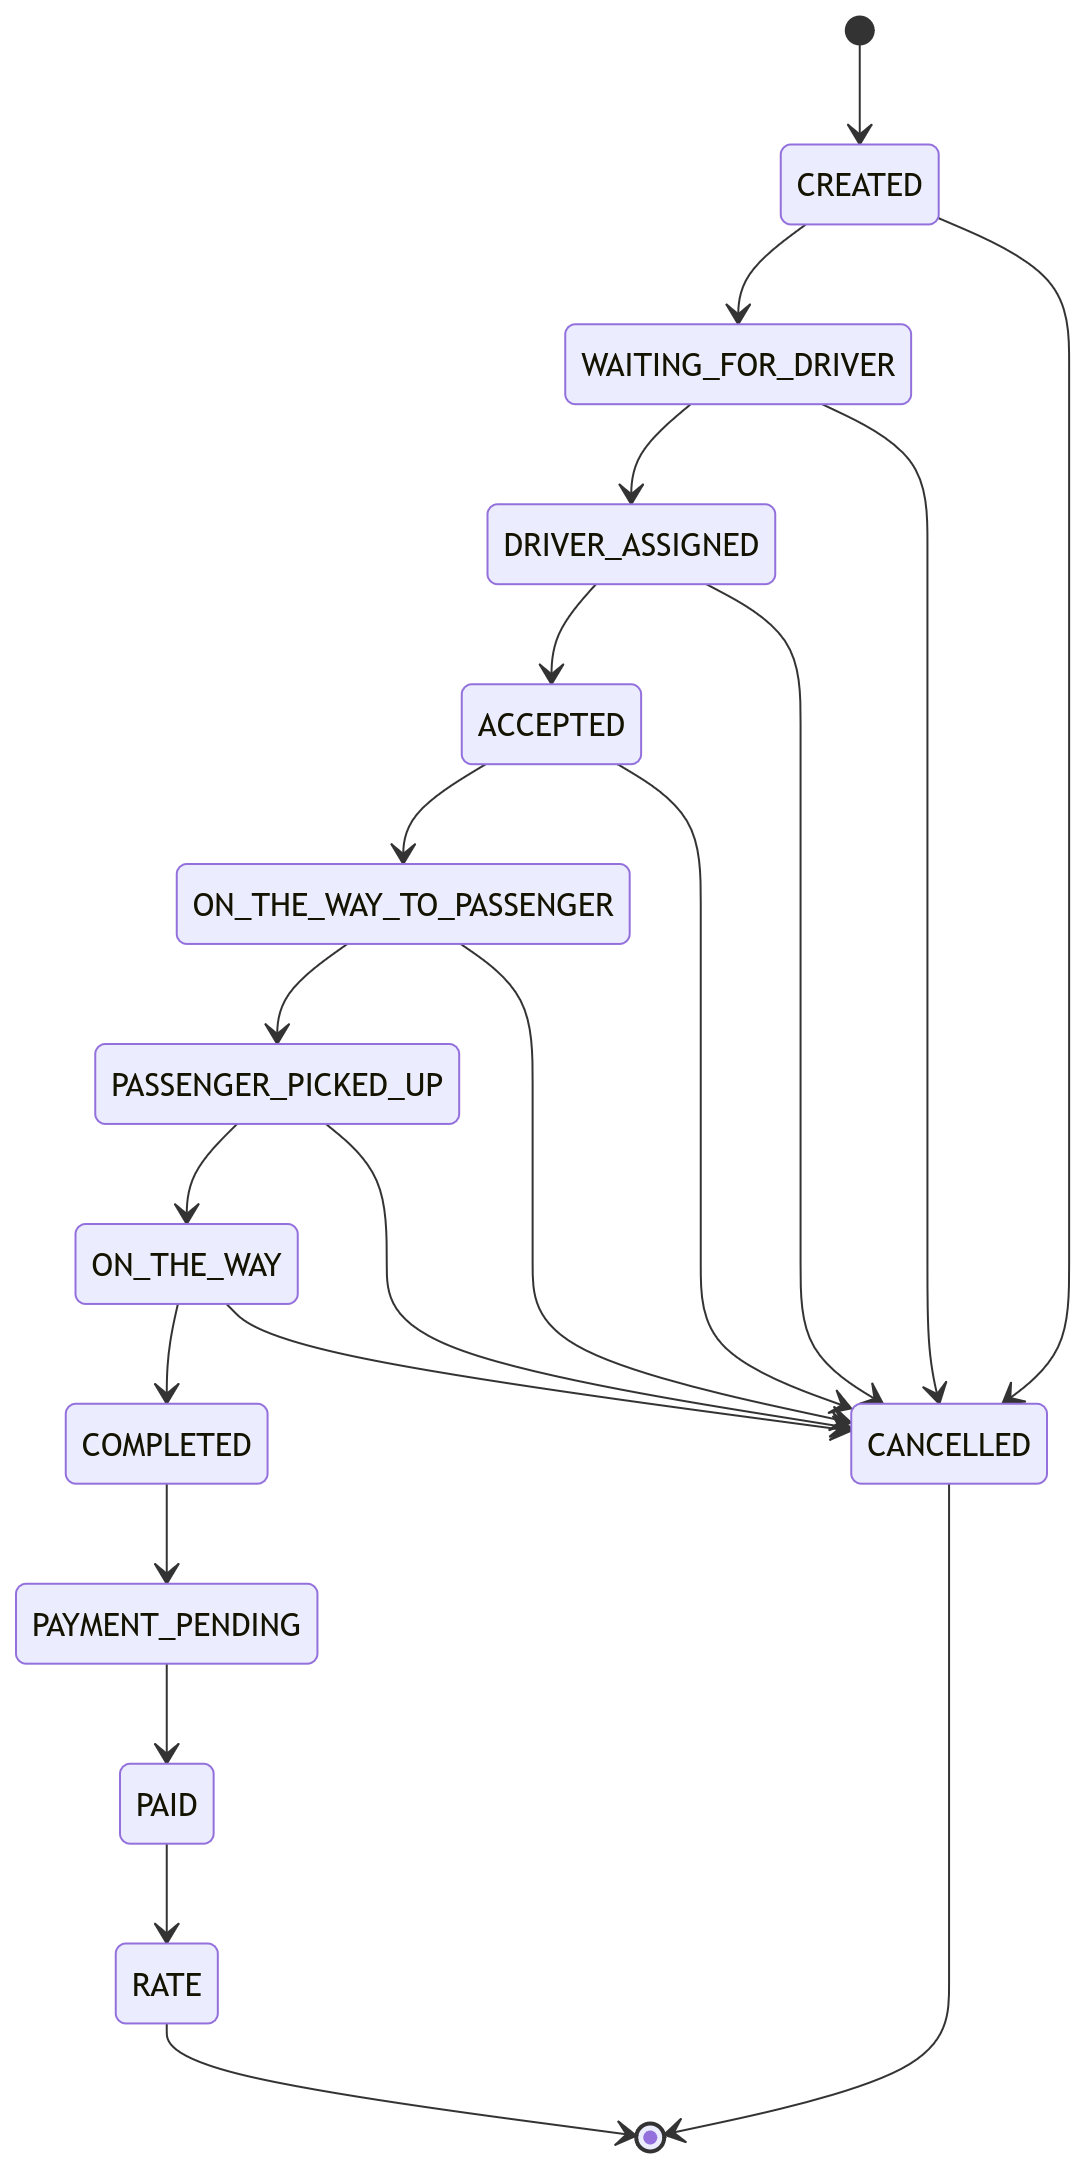
\includegraphics[width=250pt]{images/state_machine.png}
		\caption*{\gostFont Рисунок \thechaptercntr .\theimagecntr \spc {--} Диаграмма состояний поездки}
		\label{fig:StateMachine}
	\end{figure} \addtocounter{imagecntr}{1}
	
	\par \redline Переходы между состояниями строго контролируются: система проверяет допустимость перехода из текущего статуса в новый. Например, из CREATED разрешены только переходы в WAITING\_FOR\_DRIVER или CANCELLED, а из COMPLETED - только в PAYMENT\_PENDING. При определённых переходах возникают побочные эффекты: при переходе в PASSENGER\_PICKED\_UP фиксируется время подачи, при переходе в COMPLETED - время завершения поездки, а также публикуются события освобождения водителя и пассажира в Kafka.
	
	\par \redline Сервис рейтинга работает проще всех. Его основная задача - принимать оценки после завершённых поездок. Сервис рейтинга получает сообщение о завершении поездки и создаёт запись, фиксируя этот факт. После этого пассажир или водитель могут отправить POST /ratings с оценкой (от 0 до 5), комментарием и указанием, кто оценивает. Средний рейтинг считается программно: берутся последние N оценок (по умолчанию 20) и вычисляется среднее арифметическое. Это позволяет гибко настраивать количество учитываемых оценок.
	
	\par \redline Отдельно стоит сказать про каналы передачи сообщений, которые соединяют сервисы в единую систему. Всего их три: один меняет отметку "занят" у пассажира, второй - аналогично для водителя, третий передаёт информацию о завершённой поездке в сервис рейтинга. Каждый канал настроен так, чтобы сообщения не терялись и обрабатывались без дублирования.
	
	\par
}

\setcounter{subchaptercntr}{1}
\setcounter{formulacntr}{1}
\setcounter{imagecntr}{1}
\setcounter{tablecntr}{1}
